

\tikzset{every picture/.style={line width=0.75pt}} %set default line width to 0.75pt        

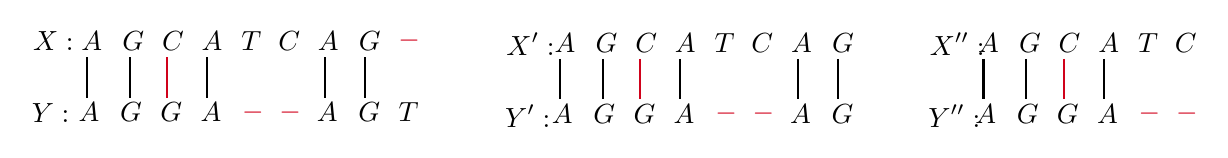
\begin{tikzpicture}[x=0.5pt,y=0.5pt,yscale=-1,xscale=1]
%uncomment if require: \path (0,113); %set diagram left start at 0, and has height of 113

%Straight Lines [id:da5184853822717996] 
\draw    (61,36) -- (61,65) ;
%Straight Lines [id:da3211316725378842] 
\draw    (92,36) -- (92,65) ;
%Straight Lines [id:da18937901909445498] 
\draw [color={rgb, 255:red, 208; green, 2; blue, 27 }  ,draw opacity=1 ]   (119,36) -- (119,65) ;
%Straight Lines [id:da5526061509479675] 
\draw    (148,36) -- (148,65) ;
%Straight Lines [id:da6049458027827691] 
\draw    (233,36) -- (233,65) ;
%Straight Lines [id:da591487642150084] 
\draw    (262,36) -- (262,65) ;
%Straight Lines [id:da8529402172351597] 
\draw    (403,37) -- (403,66) ;
%Straight Lines [id:da3161232675226988] 
\draw    (434,37) -- (434,66) ;
%Straight Lines [id:da5782198105514377] 
\draw [color={rgb, 255:red, 208; green, 2; blue, 27 }  ,draw opacity=1 ]   (461,37) -- (461,66) ;
%Straight Lines [id:da43411553560560256] 
\draw    (490,37) -- (490,66) ;
%Straight Lines [id:da8213406925141975] 
\draw    (575,37) -- (575,66) ;
%Straight Lines [id:da09244725418155642] 
\draw    (604,37) -- (604,66) ;
%Straight Lines [id:da0589047302794381] 
\draw    (709,37) -- (709,66) ;
%Straight Lines [id:da2636277707600656] 
\draw    (740,37) -- (740,66) ;
%Straight Lines [id:da8915352485728022] 
\draw [color={rgb, 255:red, 208; green, 2; blue, 27 }  ,draw opacity=1 ]   (767,37) -- (767,66) ;
%Straight Lines [id:da23944011090108752] 
\draw    (796,37) -- (796,66) ;

% Text Node
\draw (84.5,15.25) node [anchor=north west][inner sep=0.75pt]   [align=left] {$\displaystyle G$};
% Text Node
\draw (170.45,15.25) node [anchor=north west][inner sep=0.75pt]   [align=left] {$\displaystyle \textcolor[rgb]{0,0,0}{T}$};
% Text Node
\draw (113.15,15.25) node [anchor=north west][inner sep=0.75pt]   [align=left] {$\displaystyle C$};
% Text Node
\draw (225.75,15.25) node [anchor=north west][inner sep=0.75pt]   [align=left] {$\displaystyle A$};
% Text Node
\draw (255.42,15.25) node [anchor=north west][inner sep=0.75pt]   [align=left] {$\displaystyle G$};
% Text Node
\draw (141.8,15.25) node [anchor=north west][inner sep=0.75pt]   [align=left] {$\displaystyle A$};
% Text Node
\draw (82.87,66.75) node [anchor=north west][inner sep=0.75pt]   [align=left] {$\displaystyle G$};
% Text Node
\draw (111.89,66.75) node [anchor=north west][inner sep=0.75pt]   [align=left] {$\displaystyle G$};
% Text Node
\draw (224.97,66.75) node [anchor=north west][inner sep=0.75pt]   [align=left] {$\displaystyle A$};
% Text Node
\draw (254.99,66.75) node [anchor=north west][inner sep=0.75pt]   [align=left] {$\displaystyle G$};
% Text Node
\draw (140.91,66.75) node [anchor=north west][inner sep=0.75pt]   [align=left] {$\displaystyle A$};
% Text Node
\draw (284,66.75) node [anchor=north west][inner sep=0.75pt]   [align=left] {$\displaystyle T$};
% Text Node
\draw (54.85,15.25) node [anchor=north west][inner sep=0.75pt]   [align=left] {$\displaystyle A$};
% Text Node
\draw (52.85,66.75) node [anchor=north west][inner sep=0.75pt]   [align=left] {$\displaystyle A$};
% Text Node
\draw (197.1,15.25) node [anchor=north west][inner sep=0.75pt]   [align=left] {$\displaystyle C$};
% Text Node
\draw (20,15.25) node [anchor=north west][inner sep=0.75pt]   [align=left] {$\displaystyle X:$};
% Text Node
\draw (19,67.25) node [anchor=north west][inner sep=0.75pt]   [align=left] {$\displaystyle Y:$};
% Text Node
\draw (170.93,66.75) node [anchor=north west][inner sep=0.75pt]   [align=left] {$\displaystyle \textcolor[rgb]{0.82,0.01,0.11}{-}$};
% Text Node
\draw (197.95,66.75) node [anchor=north west][inner sep=0.75pt]   [align=left] {$\displaystyle \textcolor[rgb]{0.82,0.01,0.11}{-}$};
% Text Node
\draw (283.89,15.25) node [anchor=north west][inner sep=0.75pt]   [align=left] {$\displaystyle \textcolor[rgb]{0.82,0.01,0.11}{-}$};
% Text Node
\draw (426.5,16.25) node [anchor=north west][inner sep=0.75pt]   [align=left] {$\displaystyle G$};
% Text Node
\draw (512.45,16.25) node [anchor=north west][inner sep=0.75pt]   [align=left] {$\displaystyle \textcolor[rgb]{0,0,0}{T}$};
% Text Node
\draw (455.15,16.25) node [anchor=north west][inner sep=0.75pt]   [align=left] {$\displaystyle C$};
% Text Node
\draw (567.75,16.25) node [anchor=north west][inner sep=0.75pt]   [align=left] {$\displaystyle A$};
% Text Node
\draw (597.42,16.25) node [anchor=north west][inner sep=0.75pt]   [align=left] {$\displaystyle G$};
% Text Node
\draw (483.8,16.25) node [anchor=north west][inner sep=0.75pt]   [align=left] {$\displaystyle A$};
% Text Node
\draw (424.87,67.75) node [anchor=north west][inner sep=0.75pt]   [align=left] {$\displaystyle G$};
% Text Node
\draw (453.89,67.75) node [anchor=north west][inner sep=0.75pt]   [align=left] {$\displaystyle G$};
% Text Node
\draw (566.97,67.75) node [anchor=north west][inner sep=0.75pt]   [align=left] {$\displaystyle A$};
% Text Node
\draw (596.99,67.75) node [anchor=north west][inner sep=0.75pt]   [align=left] {$\displaystyle G$};
% Text Node
\draw (482.91,67.75) node [anchor=north west][inner sep=0.75pt]   [align=left] {$\displaystyle A$};
% Text Node
\draw (396.85,16.25) node [anchor=north west][inner sep=0.75pt]   [align=left] {$\displaystyle A$};
% Text Node
\draw (394.85,67.75) node [anchor=north west][inner sep=0.75pt]   [align=left] {$\displaystyle A$};
% Text Node
\draw (539.1,16.25) node [anchor=north west][inner sep=0.75pt]   [align=left] {$\displaystyle C$};
% Text Node
\draw (362,16.25) node [anchor=north west][inner sep=0.75pt]   [align=left] {$\displaystyle X':$};
% Text Node
\draw (361,68.25) node [anchor=north west][inner sep=0.75pt]   [align=left] {$\displaystyle Y':$};
% Text Node
\draw (512.93,67.75) node [anchor=north west][inner sep=0.75pt]   [align=left] {$\displaystyle \textcolor[rgb]{0.82,0.01,0.11}{-}$};
% Text Node
\draw (539.95,67.75) node [anchor=north west][inner sep=0.75pt]   [align=left] {$\displaystyle \textcolor[rgb]{0.82,0.01,0.11}{-}$};
% Text Node
\draw (732.5,16.25) node [anchor=north west][inner sep=0.75pt]   [align=left] {$\displaystyle G$};
% Text Node
\draw (818.45,16.25) node [anchor=north west][inner sep=0.75pt]   [align=left] {$\displaystyle \textcolor[rgb]{0,0,0}{T}$};
% Text Node
\draw (761.15,16.25) node [anchor=north west][inner sep=0.75pt]   [align=left] {$\displaystyle C$};
% Text Node
\draw (789.8,16.25) node [anchor=north west][inner sep=0.75pt]   [align=left] {$\displaystyle A$};
% Text Node
\draw (730.87,67.75) node [anchor=north west][inner sep=0.75pt]   [align=left] {$\displaystyle G$};
% Text Node
\draw (759.89,67.75) node [anchor=north west][inner sep=0.75pt]   [align=left] {$\displaystyle G$};
% Text Node
\draw (788.91,67.75) node [anchor=north west][inner sep=0.75pt]   [align=left] {$\displaystyle A$};
% Text Node
\draw (702.85,16.25) node [anchor=north west][inner sep=0.75pt]   [align=left] {$\displaystyle A$};
% Text Node
\draw (700.85,67.75) node [anchor=north west][inner sep=0.75pt]   [align=left] {$\displaystyle A$};
% Text Node
\draw (845.1,16.25) node [anchor=north west][inner sep=0.75pt]   [align=left] {$\displaystyle C$};
% Text Node
\draw (668,16.25) node [anchor=north west][inner sep=0.75pt]   [align=left] {$\displaystyle X'':$};
% Text Node
\draw (667,68.25) node [anchor=north west][inner sep=0.75pt]   [align=left] {$\displaystyle Y'':$};
% Text Node
\draw (818.93,67.75) node [anchor=north west][inner sep=0.75pt]   [align=left] {$\displaystyle \textcolor[rgb]{0.82,0.01,0.11}{-}$};
% Text Node
\draw (845.95,67.75) node [anchor=north west][inner sep=0.75pt]   [align=left] {$\displaystyle \textcolor[rgb]{0.82,0.01,0.11}{-}$};


\end{tikzpicture}

